% CSE440 Lab Project Report -- ACL format
% Requires acl.sty, acl_natbib.bst from https://github.com/acl-org/acl-style-files
% Compile: pdflatex -> bibtex -> pdflatex -> pdflatex
\documentclass[11pt]{article}

\usepackage[final]{acl}

\usepackage{times}
\usepackage{latexsym}
\usepackage{booktabs}
\usepackage{graphicx}
\usepackage{multirow}
\usepackage{amsmath}
\usepackage{url}
\usepackage[T1]{fontenc}
\usepackage[utf8]{inputenc}
\usepackage{microtype}
\usepackage{inconsolata}

\title{When Imbalance Handling Hurts: A Controlled Comparison of Ten
Architectures for Multi-Class Consumer Complaint Classification}

\author{
  Nabil \\
  Department of Computer Science and Engineering \\
  BRAC University \\
  \texttt{nabish0099@gmail.com}
}

\begin{document}
\maketitle

\begin{abstract}
We classify 2.02 million U.S. Consumer Financial Protection Bureau (CFPB)
complaint narratives into nine product categories, comparing ten architectures
spanning three paradigms: classical bag-of-words models over TF-IDF, six
recurrent networks over pre-trained Word2Vec embeddings, and a fine-tuned BERT
Base transformer. All ten models are trained under an identical
200{,}000-document budget and scored on an identical 303{,}213-document test
split, which makes the resulting ranking attributable to architecture rather
than to training-set size. BERT Base achieves the best test Macro F1 (0.7647),
but Logistic Regression reaches 0.7367 while running roughly 1{,}300 times
faster at inference. A probability-weighted ensemble of BERT, Random Forest and
Naive Bayes---selected on validation and scored once on test---reaches
\textbf{0.7792}, improving on BERT alone by 1.45 points for a 0.4\% increase in
inference cost, with the gain concentrated on the rarest classes. Our novelty
contribution is a controlled study of imbalance handling on a corpus with a
52.9:1 majority-to-minority ratio. Across thirteen
controlled runs we find that the standard remedy is frequently harmful: for
Logistic Regression, Naive Bayes and Bidirectional LSTM the best strategy for
minority-class F1 is \emph{no mitigation at all}, and inverse-frequency class
weighting costs the Bidirectional LSTM 7.9 F1 points on the four rarest classes.
Mitigation helps decisively only for Random Forest, the one architecture that
collapses without it. We also show that masking padded positions in the
recurrent models raises SimpleRNN Macro F1 from 0.2222 to 0.6121, indicating
that a widely reported ``vanishing-gradient'' failure of simple recurrence on
this task is partly an artefact of reading hidden states off padding.
\end{abstract}

\section{Introduction}
\label{sec:intro}

The CFPB publishes consumer complaints about financial products, and each
complaint must be routed to the responsible product team. Manual triage does not
scale to the roughly two million narratives now in the public database
\cite{cfpb2024database}, and misrouting delays regulatory response on exactly
the products where consumers have least recourse. Automatic classification of
the free-text narrative into a product category is therefore a concrete
operational problem with a public, well-documented dataset.

The task is a nine-way, single-label text classification problem. Its defining
property is severe class imbalance: \textit{Credit reporting} accounts for
59.60\% of the corpus while \textit{Payday / title / personal loan} accounts for
1.13\%, a ratio of 52.9:1. Any evaluation that leans on accuracy is therefore
uninformative, and any comparison that does not control for imbalance handling
risks measuring the mitigation rather than the model.

This work addresses three research questions.

\begin{description}
  \item[RQ1] Under an identical training budget and an identical test split,
  how do classical, recurrent and transformer architectures actually compare on
  this task, and what does the accuracy gain cost in compute?
  \item[RQ2] Does the choice of imbalance-handling strategy---class weighting,
  SMOTE oversampling, or focal loss---depend on the architecture it is applied
  to?
  \item[RQ3] How much of the reported weakness of simple recurrent models on
  long documents is attributable to sequence-padding artefacts rather than to
  the recurrence itself?
\end{description}

Our contributions are: (i) a budget-controlled comparison of ten architectures
in which every model sees the same data, removing the confound that makes many
published comparisons uninterpretable; (ii) thirteen controlled imbalance
experiments showing that mitigation is usually harmful on this corpus and helps
only the architecture that fails without it; and (iii) evidence that padding
masking, not gating, accounts for most of the gap between SimpleRNN and gated
recurrent cells here.

\section{Related Work}
\label{sec:related}

\paragraph{Text classification baselines.}
TF-IDF term weighting \cite{jones1972statistical} with a linear classifier
remains a strong baseline for topical text classification
\cite{joachims1998text}, and multinomial Naive Bayes is competitive at a
fraction of the cost \cite{mccallum1998comparison}. Random forests
\cite{breiman2001random} extend to sparse text but are sensitive to skewed
priors, as our results confirm.

\paragraph{Recurrent and contextual models.}
Simple recurrent networks \cite{elman1990finding} suffer from vanishing
gradients over long sequences, which motivated gated cells---LSTM
\cite{hochreiter1997long} and GRU \cite{cho2014learning}---and bidirectional
processing \cite{schuster1997bidirectional}. Distributed word representations
\cite{mikolov2013efficient,pennington2014glove} supply the input embeddings.
BERT \cite{devlin2019bert} replaced recurrence with pre-trained bidirectional
self-attention and defines the current strong baseline for sentence- and
document-level classification.

\paragraph{Class imbalance.}
The imbalance problem is long studied \cite{japkowicz2002class}, and modern
surveys catalogue the standard remedies \cite{johnson2019survey}: reweighting
the loss by inverse class frequency, resampling the training distribution---most
prominently SMOTE \cite{chawla2002smote}---and reshaping the loss so that easy
majority examples contribute less gradient, as in focal loss
\cite{lin2017focal}. These techniques are usually reported as improvements. Our
results indicate that on a corpus of this size the picture is considerably more
conditional, and that reporting recall alone conceals a substantial precision
cost.

\paragraph{Positioning.}
Public implementations of CFPB complaint classification that we surveyed apply
class weighting as a default and do not compare it against alternatives on a
common budget. To our knowledge, the controlled comparison in
Section~\ref{sec:novelty}---five architectures against up to four
strategies, all on identical data and scored on the identical full test
split---has not previously been reported for this dataset. We restrict this
claim to the implementations we examined; it is not a statement about all prior
work.

\section{Methodology}
\label{sec:method}

\subsection{Dataset and Exploratory Analysis}
\label{sec:data}

We use the public CFPB consumer complaint corpus distributed via Kaggle
\cite{abbasov2024kaggle,cfpb2024database}. The raw file contains 2{,}023{,}066
rows across 11 columns (2.5\,GB in memory). Every row carries narrative text, so
narrative coverage is 100\%, and there are \textbf{zero duplicate rows}. Missing
values are confined to metadata fields not used for modelling (\textit{Sub-issue}
230{,}559; \textit{Sub-product} 52{,}206; \textit{State} 7{,}344); the narrative
and target columns have none.

\paragraph{Label consolidation.}
The raw \textit{Product} field has 21 categories with substantial redundancy
(three separate credit-reporting variants, two payday-loan variants). We
consolidate these into nine coherent classes, dropping 1{,}196 rows with no
clean mapping. After preprocessing removes 450 narratives that become empty,
\textbf{2{,}021{,}420} documents remain.

\begin{table}[t]
\centering
\small
\begin{tabular}{lrr}
\toprule
\textbf{Class} & \textbf{Count} & \textbf{\%} \\
\midrule
Credit reporting            & 1{,}205{,}275 & 59.60 \\
Debt collection             &   266{,}842 & 13.20 \\
Credit card / prepaid card  &   163{,}710 &  8.10 \\
Mortgage                    &   119{,}116 &  5.89 \\
Bank account or service     &   115{,}332 &  5.71 \\
Student loan                &    44{,}241 &  2.19 \\
Money transfer / virtual cur.&   43{,}016 &  2.13 \\
Vehicle / consumer loan     &    41{,}538 &  2.05 \\
Payday / title / personal loan &  22{,}800 &  1.13 \\
\bottomrule
\end{tabular}
\caption{Nine-class distribution after consolidation. The
majority-to-minority ratio is 52.9:1.}
\label{tab:classdist}
\end{table}

Table~\ref{tab:classdist} gives the resulting distribution, visualised in
Figure~\ref{fig:classdist}. Narrative length is heavily right-skewed: mean
181.5 words, median 119, standard deviation 232.5, interquartile range
62--215, maximum 6{,}314 (Figure~\ref{fig:length}). This skew motivates our
choice of a 256-token window and, as Section~\ref{sec:padding} shows, makes
padding handling consequential.

\begin{figure}[t]
\centering
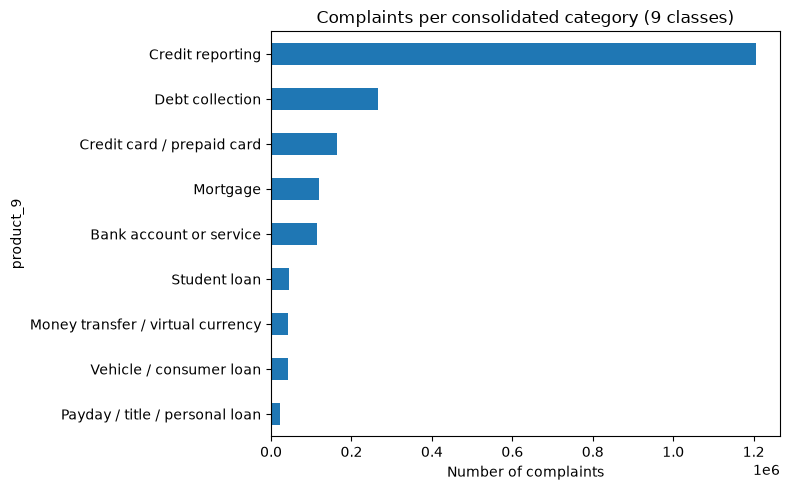
\includegraphics[width=\columnwidth]{figures/class_distribution_9.png}
\caption{Class distribution after consolidation into nine categories.}
\label{fig:classdist}
\end{figure}

\begin{figure}[t]
\centering
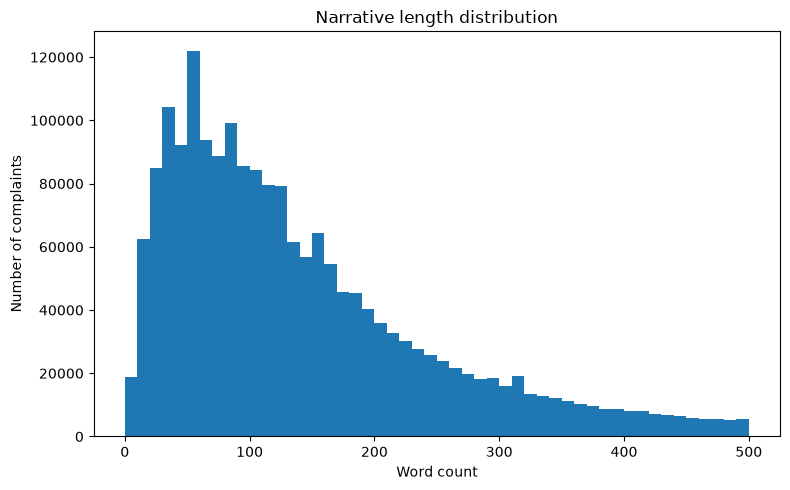
\includegraphics[width=\columnwidth]{figures/narrative_length.png}
\caption{Narrative word-count distribution. The long right tail motivates
the 256-token truncation window.}
\label{fig:length}
\end{figure}

\paragraph{Vocabulary overlap.}
Figure~\ref{fig:wordclouds} shows per-class word clouds over the cleaned
narratives. The overlaps are directly predictive of the errors reported in
Section~\ref{sec:results}: \textit{Bank account} and \textit{Money transfer}
share \textit{account}, \textit{bank}, \textit{money} and even the same
institution names, while \textit{Credit reporting} and \textit{Debt collection}
share \textit{credit report} and \textit{consumer report}. \textit{Student loan}
is lexically distinctive because servicer names (\textit{mohela},
\textit{nelnet}, \textit{navient}) appear nowhere else.

\begin{figure*}[t]
\centering
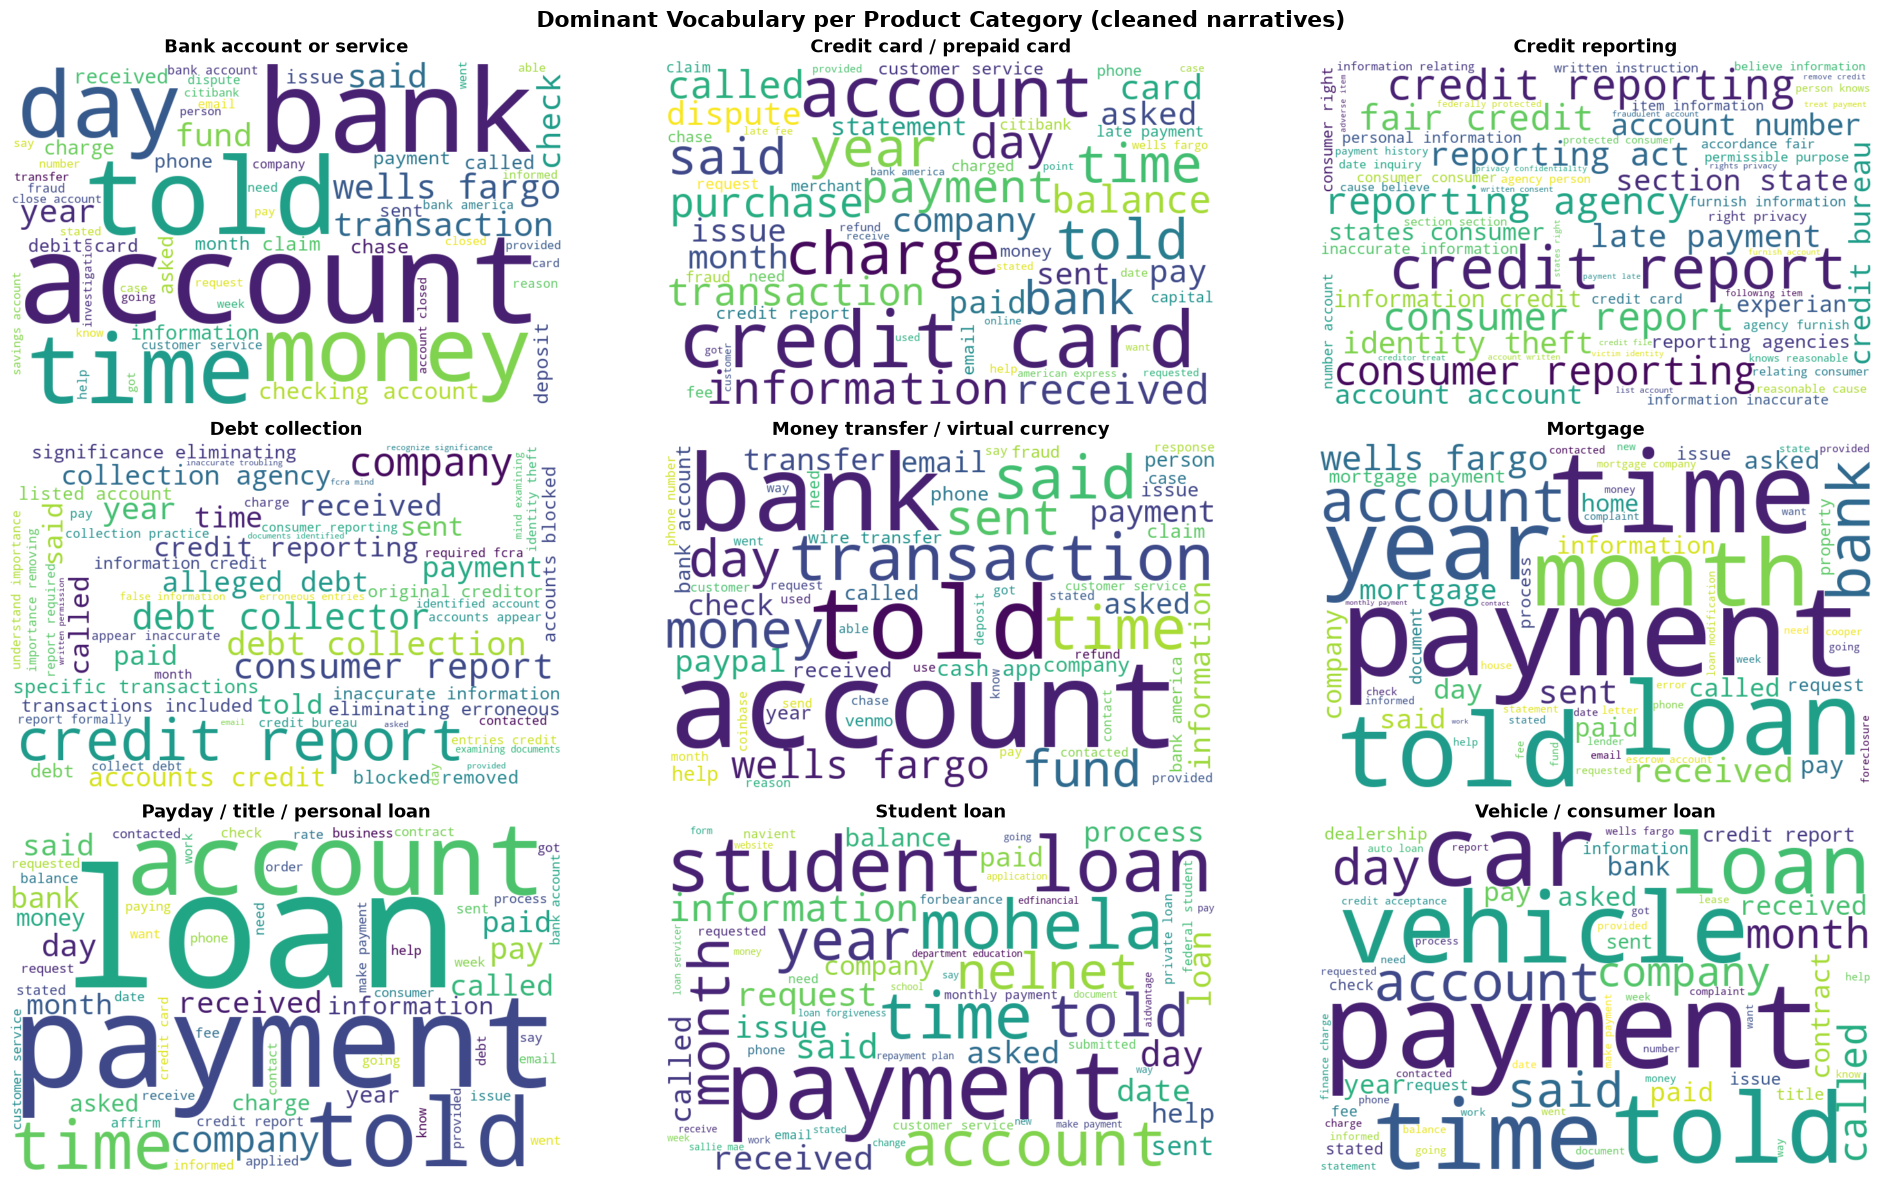
\includegraphics[width=\textwidth]{figures/wordclouds.png}
\caption{Dominant vocabulary per product category over cleaned narratives.
Shared terms between \textit{Bank account} and \textit{Money transfer}, and
between \textit{Credit reporting} and \textit{Debt collection}, anticipate the
dominant confusion corridors in Figure~\ref{fig:confusion}.}
\label{fig:wordclouds}
\end{figure*}

\subsection{Preprocessing}
\label{sec:preproc}

Because the two model families require different input properties, we build
\textbf{two preprocessing paths} from the same source text rather than forcing a
single compromise pipeline.

\textit{Contextual path} (for BERT): we strip URLs, e-mail addresses and the
CFPB's \texttt{XXXX} PII redaction markers, then normalise whitespace and
repeated punctuation. Casing, punctuation and sentence structure are
\textbf{preserved}, because BERT's WordPiece vocabulary and positional encoding
exploit them.

\textit{Classical path} (for TF-IDF and Word2Vec): we additionally lowercase,
expand contractions, remove non-alphabetic characters, drop English stopwords
and discard tokens of two characters or fewer.

The justification is empirical. The classical path reduces the median document
from 119 words to \textbf{44} and the mean from 181.5 to 70.0
(Figure~\ref{fig:preproc}), a 61\% reduction in tokens that must be carried
through a recurrent hidden state. Applying that aggressive filtering to the BERT
input would discard precisely the syntax its pre-training relies on; applying
the conservative treatment to TF-IDF would inflate the feature space with
stopwords carrying no product signal. We also verify that no non-English
narratives require handling: zero records fall below 80\% ASCII content.

\begin{figure}[t]
\centering
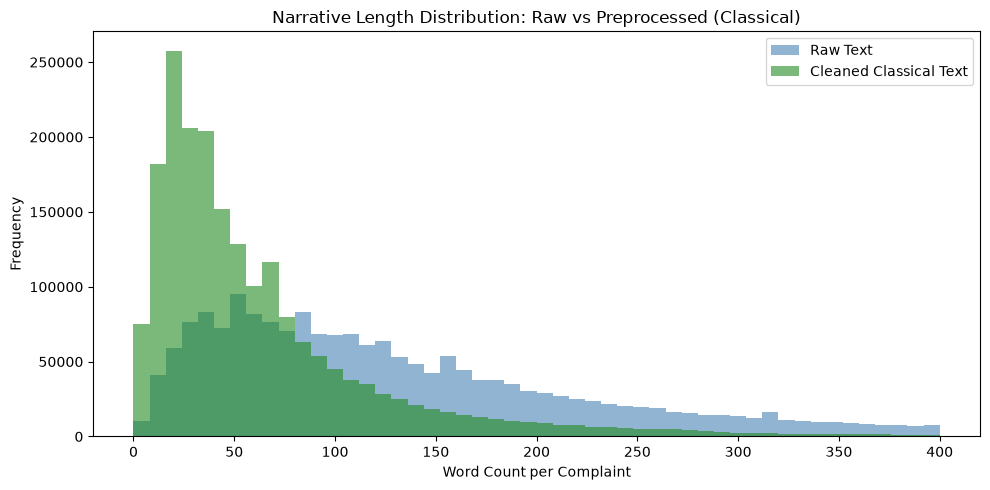
\includegraphics[width=\columnwidth]{figures/preprocessing_effect.png}
\caption{Word-count distribution before and after classical preprocessing.
The median falls from 119 to 44 tokens.}
\label{fig:preproc}
\end{figure}

\subsection{Train/Validation/Test Split}
\label{sec:split}

We split 70/15/15 into 1{,}414{,}994 training, 303{,}213 validation and
303{,}213 test documents. The split is \textbf{stratified} on the nine-class
label and seeded (\texttt{random\_state=42}), making it exactly reproducible. We
verify stratification empirically rather than assuming it: \textit{Credit
reporting} occupies 59.60\% of all three partitions and \textit{Payday loan}
1.13\% of all three (Figure~\ref{fig:strat}). All fitting---the TF-IDF
vocabulary, the Word2Vec embeddings and every classifier---uses training data
only; validation and test are transform-only, so no target leakage is possible.

\begin{figure}[t]
\centering
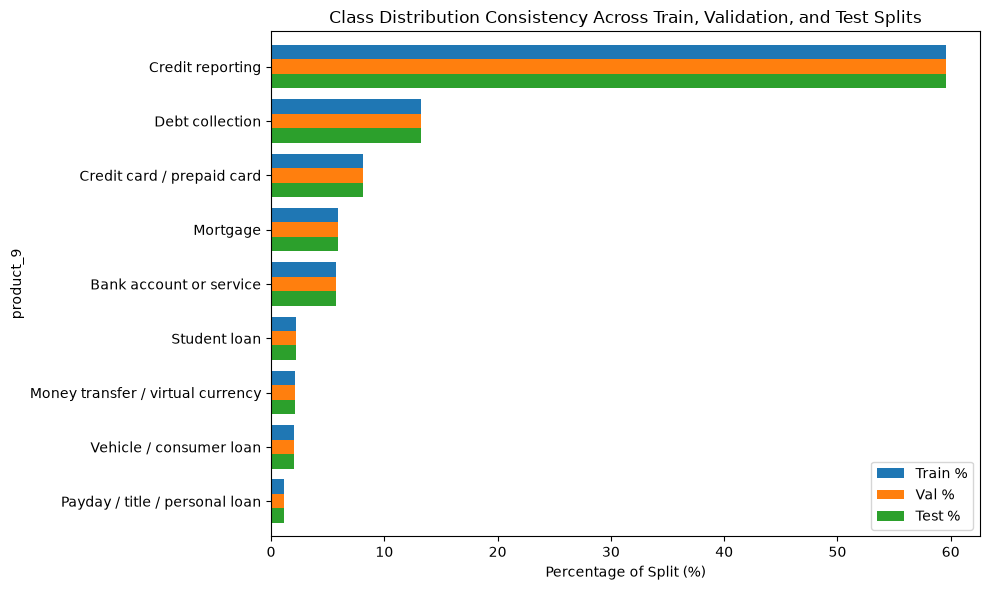
\includegraphics[width=\columnwidth]{figures/split_stratification.png}
\caption{Class proportions across the three splits, confirming stratification.}
\label{fig:strat}
\end{figure}

\subsection{Word Representations}
\label{sec:repr}

We implement three representations, satisfying the requirement of at least two
of TF-IDF, Word2Vec and GloVe.

\textbf{TF-IDF} \cite{jones1972statistical}: 25{,}000 features over unigrams and
bigrams, sublinear term-frequency scaling, \texttt{min\_df=5},
\texttt{max\_df=0.85}. Fitted on the full training split, giving a
$1{,}414{,}994 \times 25{,}000$ sparse matrix with 103{,}726{,}073 non-zero
entries (0.29\% density). The highest mean-weight features are
\textit{credit}, \textit{account}, \textit{report}, \textit{information}.

\textbf{Word2Vec} \cite{mikolov2013efficient}: 100-dimensional CBOW embeddings
trained in-domain on the full training corpus for five epochs
(\texttt{min\_count=5}), via Gensim \cite{rehurek2010gensim}. In-domain training
is preferable to pre-trained GloVe vectors here because financial-complaint
vocabulary (\textit{escrow}, \textit{chargeback}, servicer names) is poorly
covered by general-corpus embeddings. These vectors initialise the recurrent
models' embedding layer, which is then fine-tuned.

\textbf{WordPiece}: BERT's own subword vocabulary, used for the transformer.

\subsection{Model Architectures and Protocol}
\label{sec:models}

\paragraph{Fixed training budget.}
Fine-tuning BERT over 1.41M documents is not tractable on a single consumer GPU
within this project's timeframe, so the transformer sets the ceiling for the
whole comparison. We therefore train \textbf{every} architecture on the same
stratified 200{,}000-document subsample and score every architecture on the
\textbf{full} 303{,}213-document test split. Representations are still fitted on
the full 1.41M training split; only the classifier fitting budget is capped.
This is the central methodological decision of the study: without it, a ranking
would confound architecture with training-set size.

\paragraph{Classical models.}
Logistic Regression (lbfgs, \texttt{max\_iter=1000}), Multinomial Naive Bayes,
and Random Forest (50 trees), via scikit-learn \cite{pedregosa2011scikit}.

\paragraph{Recurrent models.}
A single configurable module implements SimpleRNN, GRU and LSTM in
unidirectional and bidirectional form (six architectures), in PyTorch
\cite{paszke2019pytorch}. Inputs are 256-token padded sequences initialised with
the Word2Vec matrix. Crucially, the final hidden state is read through
\texttt{pack\_padded\_sequence}, so each sequence contributes its true final
token rather than a state advanced through padding
(Section~\ref{sec:padding}). Training uses Adam, gradient-norm clipping at 1.0,
and four epochs, with the reported epoch selected on validation Macro F1.

\paragraph{Transformer.}
\texttt{bert-base-uncased} \cite{devlin2019bert} via Hugging Face Transformers
\cite{wolf2020transformers}, fine-tuned for two epochs with AdamW, batch size
32, and bfloat16 mixed precision.

\paragraph{Hyperparameter tuning.}
Every model is tuned over at least three configurations against validation Macro
F1, for \textbf{30 tuning runs} in total: nine classical (three each), eighteen
recurrent (three configurations $\times$ six architectures) and three BERT
learning rates $\{2,3,5\}\times10^{-5}$. All runs are recorded in the notebook's
Section 3.8 table and summarised in Figure~\ref{fig:tuning}. BERT's optimum is
the lowest learning rate ($2\times10^{-5}$, 0.7647); the two higher rates are
indistinguishable from each other (0.7480 and 0.7499).

\begin{figure}[t]
\centering
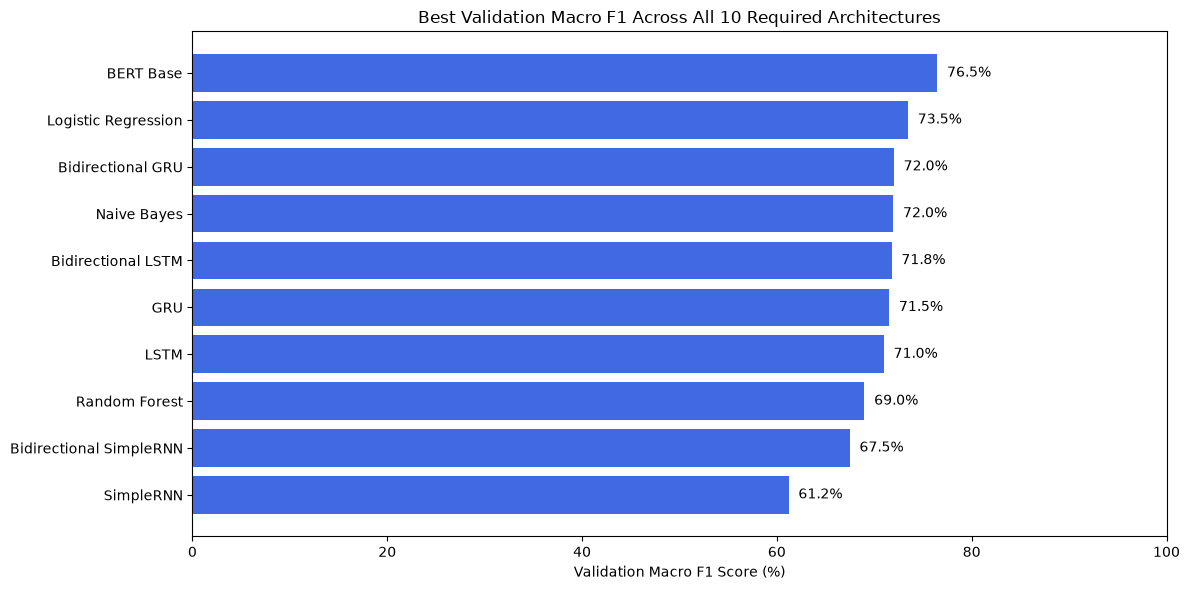
\includegraphics[width=\columnwidth]{figures/tuning_overview.png}
\caption{Best validation Macro F1 per architecture across all 30 tuning runs.}
\label{fig:tuning}
\end{figure}

\section{Results}
\label{sec:results}

\subsection{Model Comparison}

\begin{table*}[t]
\centering
\small
\begin{tabular}{clrrrrr}
\toprule
\textbf{\#} & \textbf{Model} & \textbf{Macro F1} & \textbf{Accuracy} &
\textbf{Weighted F1} & \textbf{Train (s)} & \textbf{Infer (s)} \\
\midrule
1  & BERT Base $\dagger$        & \textbf{0.7647} & 0.8562 & 0.8613 & 1678.1 & 267.3 \\
2  & Logistic Regression        & 0.7367 & 0.8390 & 0.8468 & 34.5 & \textbf{0.2} \\
3  & GRU                        & 0.7274 & 0.8326 & 0.8420 & 77.2 & 5.8 \\
4  & Bidirectional GRU          & 0.7234 & 0.8267 & 0.8376 & 130.6 & 8.4 \\
5  & Naive Bayes                & 0.7211 & 0.8329 & 0.8357 & \textbf{0.1} & 0.2 \\
6  & Bidirectional LSTM         & 0.7173 & 0.8175 & 0.8274 & 139.1 & 9.2 \\
7  & LSTM                       & 0.7110 & 0.8180 & 0.8276 & 78.2 & 5.8 \\
8  & Random Forest              & 0.6920 & 0.8121 & 0.8197 & 31.0 & 0.8 \\
9  & Bidirectional SimpleRNN    & 0.6600 & 0.7824 & 0.7944 & 124.2 & 8.9 \\
10 & SimpleRNN $\ddagger$       & 0.5685 & 0.6722 & 0.6943 & 80.5 & 5.9 \\
\bottomrule
\end{tabular}
\caption{Held-out test results for all ten architectures. Every model was
trained on the same 200{,}000-document budget and scored on the same
303{,}213-document test split. $\dagger$ best-performing; $\ddagger$
worst-performing. Inference time is a pure prediction pass over the full test
set, reported separately from training.}
\label{tab:main}
\end{table*}

Table~\ref{tab:main} reports the main comparison, visualised in
Figure~\ref{fig:comparison}. \textbf{BERT Base is the best-performing model}
(Macro F1 0.7647) and \textbf{SimpleRNN the worst} (0.5685), a spread of 19.62
points.

\begin{figure}[t]
\centering
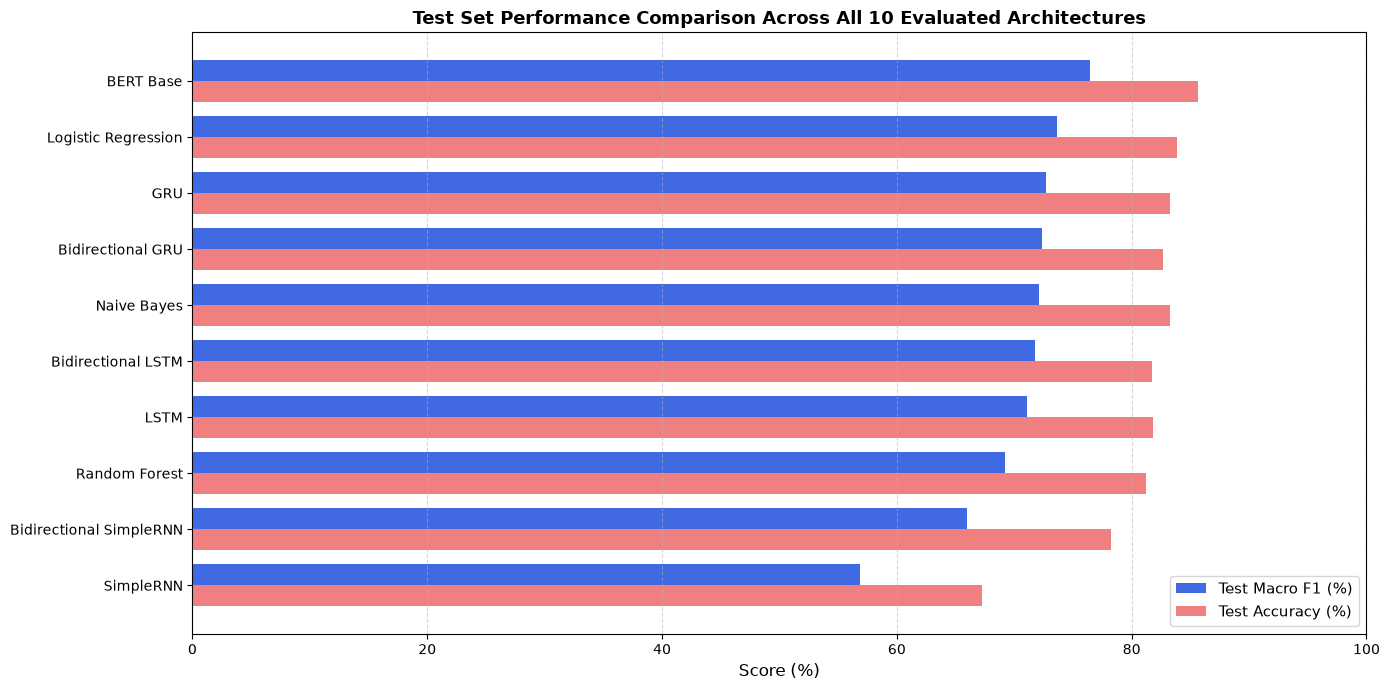
\includegraphics[width=\columnwidth]{figures/model_comparison.png}
\caption{Test Macro F1 and accuracy across all ten architectures.}
\label{fig:comparison}
\end{figure}

Three findings deserve emphasis.

\paragraph{The accuracy gain is expensive.}
BERT exceeds Logistic Regression by 2.80 Macro F1 points while requiring
$49\times$ the training time and $1{,}336\times$ the inference time. Logistic
Regression classifies all 303{,}213 test documents in 0.2 seconds; BERT needs
4.5 minutes. Naive Bayes reaches 0.7211---within 4.4 points of BERT---from
0.1 seconds of training. For a routing system operating at CFPB volume, the
linear baseline is the stronger engineering choice unless the 2.8-point gain
carries specific regulatory value.

\paragraph{Sequence modelling does not pay for itself.}
Every recurrent architecture is beaten by Logistic Regression. On a task where
the discriminative signal is largely lexical---the word clouds in
Figure~\ref{fig:wordclouds} show product vocabulary is highly separable---word
order contributes little that bag-of-bigrams does not already capture.

\paragraph{Bidirectionality helps only ungated cells.}
SimpleRNN gains 9.15 points from bidirectional processing, but LSTM gains only
0.63 and GRU \textbf{loses} 0.40, both within the $\pm0.85$-point run-to-run
variance we measured for these models. A gated cell already propagates
information across the sequence effectively enough that a reverse pass adds
nothing, while costing roughly 70\% more training time and twice the parameters.

\subsection{Padding Artefacts in Recurrent Models}
\label{sec:padding}

An earlier iteration of this pipeline read the final hidden state directly off
the padded sequence. Because the classical preprocessing path reduces the median
narrative to 44 tokens while sequences are padded to 256, that hidden state was
advanced through roughly 200 \texttt{<PAD>} steps before being classified. Under
that configuration SimpleRNN reached Macro F1 0.2222 and its accuracy fell below
the $1/9$ random baseline. Masking padded positions with
\texttt{pack\_padded\_sequence} raises the same architecture, on the same data
and configuration, to \textbf{0.6121} validation Macro F1---a $2.8\times$
improvement obtained without changing the model.

This has an interpretive consequence. The gap between SimpleRNN and gated cells
narrows from 51.7 points to 10.3 points once padding is masked, so most of the
apparent advantage of gating on this task was a padding artefact rather than a
property of the recurrence.

\subsection{Error Analysis}

\begin{figure*}[t]
\centering
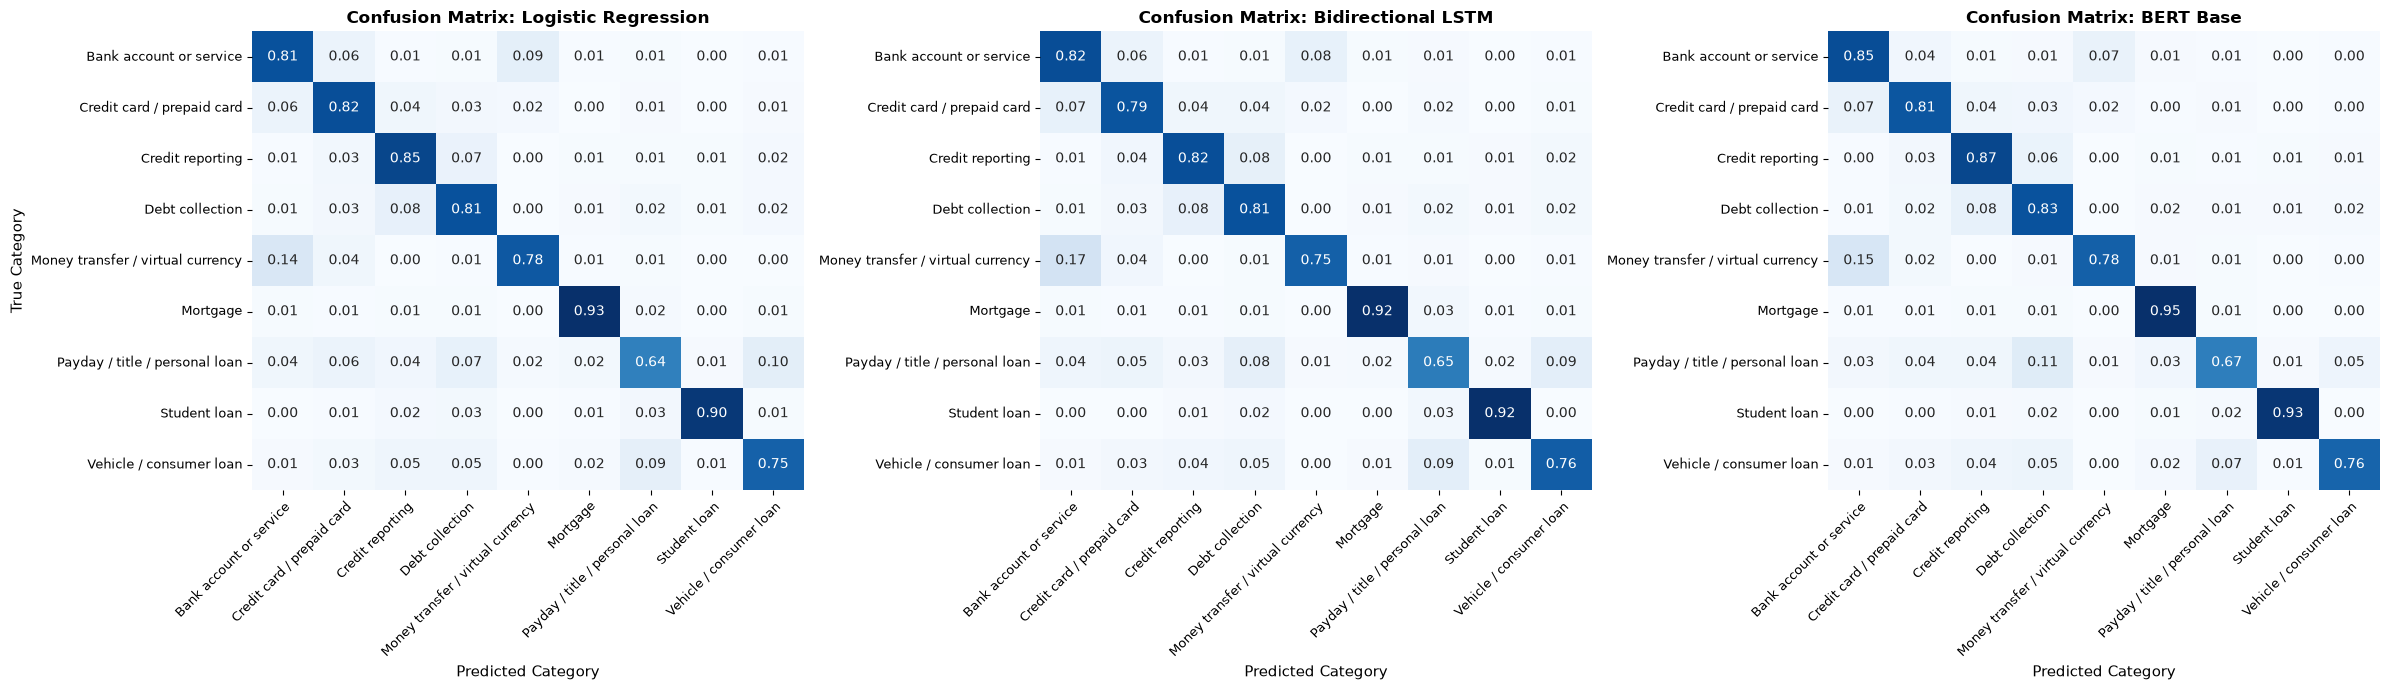
\includegraphics[width=\textwidth]{figures/confusion_matrices.png}
\caption{Row-normalised confusion matrices for one model from each paradigm.}
\label{fig:confusion}
\end{figure*}

Figure~\ref{fig:confusion} shows row-normalised confusion matrices. The dominant
error is consistent across paradigms and is exactly the one the EDA predicts:
\textbf{14--17\% of \textit{Money transfer} complaints are predicted as
\textit{Bank account or service}}, the two classes whose word clouds overlap
most. \textit{Payday loan} is the hardest class everywhere (recall 0.64--0.67),
consistent with it being rarest at 1.13\%, while \textit{Mortgage} is easiest
(0.93--0.95) on a distinctive vocabulary.

BERT's advantage is qualitative, not merely quantitative. It nearly halves the
\textit{Payday}$\rightarrow$\textit{Vehicle loan} confusion (0.05 versus 0.10 for
Logistic Regression) but \emph{worsens}
\textit{Payday}$\rightarrow$\textit{Debt collection} (0.11 versus 0.07). Context
helps it separate loan products by their described terms, while making it more
willing to assign a complaint describing collection activity to the collection
class.

% Generated from ensemble_results.json by pipeline/gen_tex.py
% Generated by pipeline/gen_tex.py -- do not edit by hand.
\subsection{Ensemble of the Best-Performing Models}
\label{sec:ensemble}

Section~\ref{sec:results} showed that the three paradigms make qualitatively different errors, which is the precondition for a useful ensemble. We searched 1506 candidate combinations (hard and soft voting, uniform and validation-F1 weighting, 3--9 members) \textbf{on the validation split}, then scored the single winning configuration on the test split once. Selecting members by test performance would report a gain that does not generalise.

The selected system is soft voting with val-F1 weighting over 3 members: \textbf{BERT Base}, \textbf{Random Forest}, \textbf{Naive Bayes}.

\begin{table}[t]
\centering
\small
\begin{tabular}{lr}
\toprule
\textbf{System} & \textbf{Test Macro F1} \\
\midrule
BERT Base (best single) & 0.7647 \\
Ensemble & \textbf{0.7792} \\
\midrule
Difference & +1.45 pp \\
\bottomrule
\end{tabular}
\caption{Ensemble versus the best single model. Members were selected on validation (macro F1 0.7795) and the test split was scored once.}
\label{tab:ensemble}
\end{table}

\begin{table}[t]
\centering
\small
\begin{tabular}{lrr}
\toprule
\textbf{Member} & \textbf{Disagree} & \textbf{Own F1} \\
\midrule
Random Forest & 14.0\% & 0.6920 \\
Naive Bayes & 13.7\% & 0.7211 \\
\bottomrule
\end{tabular}
\caption{Ensemble member diversity: fraction of test documents on which each member disagrees with BERT Base. Decorrelation, not individual strength, is what earns a place in the vote.}
\label{tab:diversity}
\end{table}

\begin{table}[t]
\centering
\small
\begin{tabular}{lrrr}
\toprule
\textbf{Class} & \textbf{BERT Base} & \textbf{Ens.} & $\Delta$ \\
\midrule
Payday / title / personal loan & 0.5401 & 0.5735 & +3.34 \\
Vehicle / consumer loan & 0.6391 & 0.6554 & +1.63 \\
Money transfer / virtual currency & 0.7454 & 0.7608 & +1.54 \\
Student loan & 0.7912 & 0.8202 & +2.90 \\
Bank account or service & 0.8157 & 0.8292 & +1.34 \\
Mortgage & 0.8981 & 0.9004 & +0.23 \\
Credit card / prepaid card & 0.7679 & 0.7762 & +0.83 \\
Debt collection & 0.7693 & 0.7767 & +0.74 \\
Credit reporting & 0.9156 & 0.9204 & +0.48 \\
\bottomrule
\end{tabular}
\caption{Per-class F1, ordered from rarest to most common class.}
\label{tab:ensembleperclass}
\end{table}

The gain concentrates on the rare classes (+2.35 pp mean over the four smallest, against +0.57 pp over the four largest), which is the desirable direction: rare classes are where individual models are least confident and a vote has most to correct.

An ensemble pays the inference cost of every member: 268.3\,s over the test set against 267.3\,s for BERT Base alone (1.00$\times$).

That overhead is negligible, because the two added members are the cheapest models in the study: the ensemble costs 1.0\,s more than BERT Base alone across 303{,}213 documents, a 0.4\% increase, for +1.45 pp of Macro F1. Unlike the accuracy/latency trade of Table~\ref{tab:main}, there is no trade-off to weigh here: the ensemble dominates its strongest member at essentially equal cost.


\subsection{Imbalance Handling}
\label{sec:novelty}

\begin{table}[t]
\centering
\small
\begin{tabular}{llrr}
\toprule
\textbf{Model} & \textbf{Strategy} & \textbf{Macro F1} & \textbf{Min-4 F1} \\
\midrule
\multirow{3}{*}{Log.\ Reg.}
 & None            & \textbf{0.7703} & \textbf{0.6829} \\
 & Class Weighting & 0.7367 & 0.6347 \\
 & SMOTE           & 0.7348 & 0.6353 \\
\midrule
\multirow{2}{*}{Naive Bayes}
 & None            & \textbf{0.7211} & \textbf{0.6304} \\
 & SMOTE           & 0.6873 & 0.5853 \\
\midrule
\multirow{3}{*}{Rand.\ Forest}
 & None            & 0.5702 & 0.3389 \\
 & Class Weighting & 0.6920 & 0.5820 \\
 & SMOTE           & \textbf{0.7142} & \textbf{0.6198} \\
\midrule
\multirow{3}{*}{Bi-LSTM}
 & None            & \textbf{0.7627} & \textbf{0.6718} \\
 & Class Weighting & 0.7088 & 0.5931 \\
 & Focal Loss      & 0.7090 & 0.6010 \\
\midrule
\multirow{2}{*}{BERT Base}
 & Class Weighting & \textbf{0.7647} & \textbf{0.6789} \\
 & Focal Loss      & 0.7506 & 0.6736 \\
\bottomrule
\end{tabular}
\caption{Imbalance-handling comparison. Min-4 F1 is the mean F1 over the four
rarest classes. All arms use the identical 200{,}000-document budget and the
identical full test split; only the strategy varies. Naive Bayes exposes no
class-weight parameter.}
\label{tab:novelty}
\end{table}

Table~\ref{tab:novelty} reports thirteen controlled runs, visualised in
Figure~\ref{fig:imbalance}. The metric of interest is Min-4 F1, the mean F1 over
the four rarest classes, since these are what mitigation exists to improve.

\begin{figure}[t]
\centering
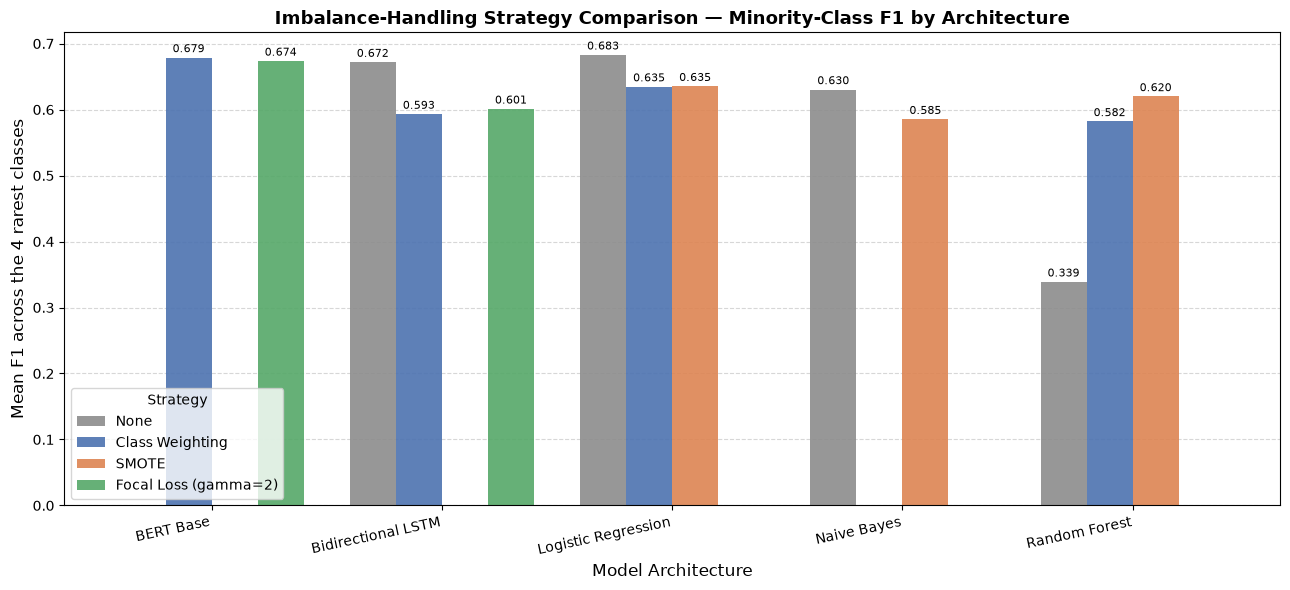
\includegraphics[width=\columnwidth]{figures/imbalance_comparison.png}
\caption{Minority-class F1 by architecture and imbalance strategy.}
\label{fig:imbalance}
\end{figure}

\paragraph{Mitigation is usually harmful.}
In three of the five architectures---Logistic Regression, Naive Bayes and
Bidirectional LSTM---the best strategy for minority-class F1 is \textbf{no
mitigation at all}. Class weighting costs the Bidirectional LSTM 7.9 points and
Logistic Regression 4.8 points on precisely the classes it is intended to
rescue. The mechanism is a precision/recall trade: inverse-frequency weighting
raises minority recall while sharply reducing minority precision, and F1
penalises the exchange. Reporting recall alone, as is common, conceals this.

\paragraph{Mitigation rescues only the model that fails without it.}
Random Forest is the sole architecture that benefits decisively, gaining 28.1
points of Min-4 F1 from SMOTE and 24.3 from class weighting. Untreated it scores
0.3389, because a depth-limited forest splitting on a 59.6\% majority rarely
isolates minority regions at all. This suggests reframing imbalance handling as
\emph{compensation for an architecture that cannot absorb skew}, rather than as
a technique that improves an architecture that can.

\paragraph{The hypothesis of architecture-dependence is not supported.}
We expected focal loss to win for deep models and SMOTE for linear ones. Neither
holds. Focal loss loses to class weighting on BERT (0.6736 versus 0.6789) and to
no mitigation on Bi-LSTM (0.6010 versus 0.6718); SMOTE loses on both linear
models and wins only on the non-linear Random Forest. Because ``no mitigation''
wins for both a classical and a deep model, the winning strategies overlap
across paradigms and the architecture-conditioned claim must be rejected.

\paragraph{Cost.}
SMOTE expands the training set from 200{,}000 to 1{,}072{,}881 rows. Its best
result (Random Forest, 0.6198) is still 6.3 points below what Logistic
Regression achieves with no mitigation in 28 seconds. On this corpus, the most
elaborate rebalancing applied to the model that needs it most does not reach the
simplest model left alone.

\section{Conclusion}
\label{sec:conclusion}

We compared ten architectures for nine-way CFPB complaint classification under
a fixed training budget and a common test split. BERT Base is the most accurate
(Macro F1 0.7647) but Logistic Regression retains 96\% of that performance at
roughly $1/1300$ of the inference cost, and every recurrent model is beaten by
the linear baseline---evidence that this task is predominantly lexical.

A validation-selected soft-voting ensemble of BERT, Random Forest and Naive
Bayes reaches 0.7792, and its composition is instructive: the two added members
rank eighth and fifth individually, but disagree with BERT on 14.0\% and 13.7\%
of documents, more than any recurrent model. Decorrelation, not individual
accuracy, earns a place in the vote. Because both are among the cheapest models
in the study, the ensemble improves on BERT by 1.45 points for one additional
second of inference across 303{,}213 documents.

Our main contribution is negative and, we think, useful: on a corpus with a
52.9:1 imbalance ratio, standard imbalance handling degraded minority-class F1
for three of five architectures. It helped decisively only for Random Forest,
the one model that collapses without it. We also showed that masking padded
positions accounts for most of the apparent superiority of gated cells over
simple recurrence here.

\paragraph{Limitations.}
The 200{,}000-document budget, while applied uniformly, is 14\% of the available
training data; absolute scores would rise with more data, though the relative
ranking held between validation and test throughout. We did not seed PyTorch
initialisation, and measured run-to-run variance of approximately $\pm0.85$
Macro F1 points on the recurrent models; differences smaller than this---notably
the bidirectional effects on GRU and LSTM---should be treated as ties. Focal
loss was evaluated at $\gamma=2$ with inverse-frequency $\alpha$ weighting only,
so our comparison isolates the focal modulation on top of class weighting rather
than focal loss in isolation. Finally, all findings are specific to this corpus
and label scheme.

\paragraph{Future work.}
Three directions follow. First, threshold tuning per class is a cheaper lever
than reweighting and directly targets the precision/recall trade we identified.
Second, the \textit{Money transfer}/\textit{Bank account} confusion is a label
schema question as much as a modelling one and may warrant a merged or
hierarchical target. Third, an ensemble of the linear and transformer
models---which make qualitatively different errors---should be tested, since
their disagreement pattern suggests complementary strengths.

\section*{Reproducibility}

All results are produced by a staged pipeline with disk-cached artefacts;
no metric is hardcoded. The random seed is 42 for all splits and classical
models. Experiments ran on an NVIDIA RTX 4070 Ti SUPER (16\,GB), total wall
clock approximately 3.5 hours. Figures were produced with Matplotlib
\cite{hunter2007matplotlib} and NumPy \cite{harris2020array}; SMOTE via
imbalanced-learn \cite{lemaitre2017imbalanced}.

\bibliography{custom}
\bibliographystyle{acl_natbib}

\appendix
\section{A Causal-Decoder Arm: Qwen2.5-1.5B with LoRA}
\label{sec:qwen}

The ten systems compared in Section~\ref{sec:results} span classical, recurrent
and bidirectional-encoder paradigms. A fourth paradigm --- the modern
causal-decoder small language model --- was explored separately, and we report
it here rather than in Table~\ref{tab:main} for a reason we make explicit below.

\subsection{Method}

Qwen2.5-1.5B \cite{yang2024qwen2} was adapted for nine-way classification with
Low-Rank Adaptation \cite{hu2021lora}: rank $r=16$, $\alpha=32$, dropout $0.05$,
applied to all attention and MLP projections
(\texttt{q,k,v,o,gate,up,down\_proj}) with the classification head left
trainable. This updates roughly $1.2\%$ of the 1.54B backbone. Training used
class-weighted cross-entropy, AdamW at $2\times10^{-4}$ with linear warmup over
the first $10\%$ of steps, batch size 16 with two-step gradient accumulation,
\texttt{bfloat16} autocast, and two epochs. Sequences were truncated to 256
WordPiece-equivalent tokens, matching the BERT arm. Because Qwen is a causal
decoder, the sequence representation is pooled at the last non-padding position,
so padding is applied on the right and \texttt{pad\_token\_id} is set explicitly.

\subsection{Why this result is not in the main table}

The run was carried out on a separately prepared copy of the corpus with its own
label mapping, and was scored on a \textbf{5,000-document} test subset rather
than the 303,213-document split used by every other system in this paper. The
training budget for that copy was not recorded, so we cannot confirm it matched
the 200,000-row budget that makes Table~\ref{tab:main} a controlled comparison.
Placing the resulting figure in that table would break the one property the
table exists to guarantee.

The size of the risk is measurable, and it is not negligible. Using the stored
test predictions of three of our own models, we resampled 5,000-document subsets
of the real test split 30 times and recomputed macro F1 (Table~\ref{tab:subset}).
A subset drawn \emph{proportionally} to the true class priors is essentially
unbiased, but carries a standard deviation of about $1.1$ points --- wider than
the margin separating most adjacent rows of Table~\ref{tab:main}. A
\emph{class-balanced} subset of the same size inflates macro F1 by roughly six
points, because the rare classes whose precision collapses under a $52.9{:}1$
prior are no longer rare.

\begin{table}[t]
\centering
\small
\begin{tabular}{lccc}
\toprule
\textbf{Model} & \textbf{Full} & \textbf{Prop. 5k} & \textbf{Bal. 5k} \\
\midrule
BERT Base           & 0.7647 & $0.766 \pm 0.011$ & $0.824 \pm 0.005$ \\
Logistic Regression & 0.7367 & $0.739 \pm 0.007$ & $0.810 \pm 0.005$ \\
Random Forest       & 0.6920 & $0.690 \pm 0.008$ & $0.751 \pm 0.006$ \\
\bottomrule
\end{tabular}
\caption{Test macro F1 on the full 303,213-document split against 5,000-document
subsets, over 30 resamples. Proportional subsets are unbiased but noisy;
class-balanced subsets are inflated by about six points. This is why a
subset-scored result cannot be quoted alongside full-split results.}
\label{tab:subset}
\end{table}

We cannot determine from the recorded artefacts which of the two regimes the
Qwen subset followed. Its normalised confusion matrix (Figure~\ref{fig:qwencm})
implies an accuracy of $0.80$ if the subset was balanced and $0.87$ if it was
proportional, and the reported accuracy of $0.828$ falls between them.

\subsection{Provisional result}

Subject to those caveats, the run reached a macro F1 of approximately $0.74$ and
an accuracy of approximately $0.83$ on its own 5,000-document subset, with a
per-document inference cost roughly an order of magnitude above BERT's --- the
expected consequence of a 1.5B decoder against a 110M encoder. The confusion
structure in Figure~\ref{fig:qwencm} is qualitatively consistent with the
encoder models: \emph{Credit reporting} is recovered most reliably, the
\emph{Debt collection} $\rightarrow$ \emph{Credit reporting} corridor is the
dominant off-diagonal term, and \emph{Payday / personal loan} is the weakest
class. We therefore treat the arm as evidence that a LoRA-adapted decoder is
\emph{competitive} on this task, and not as a measured ranking against the ten
systems in Table~\ref{tab:main}.

\begin{figure}[t]
\centering
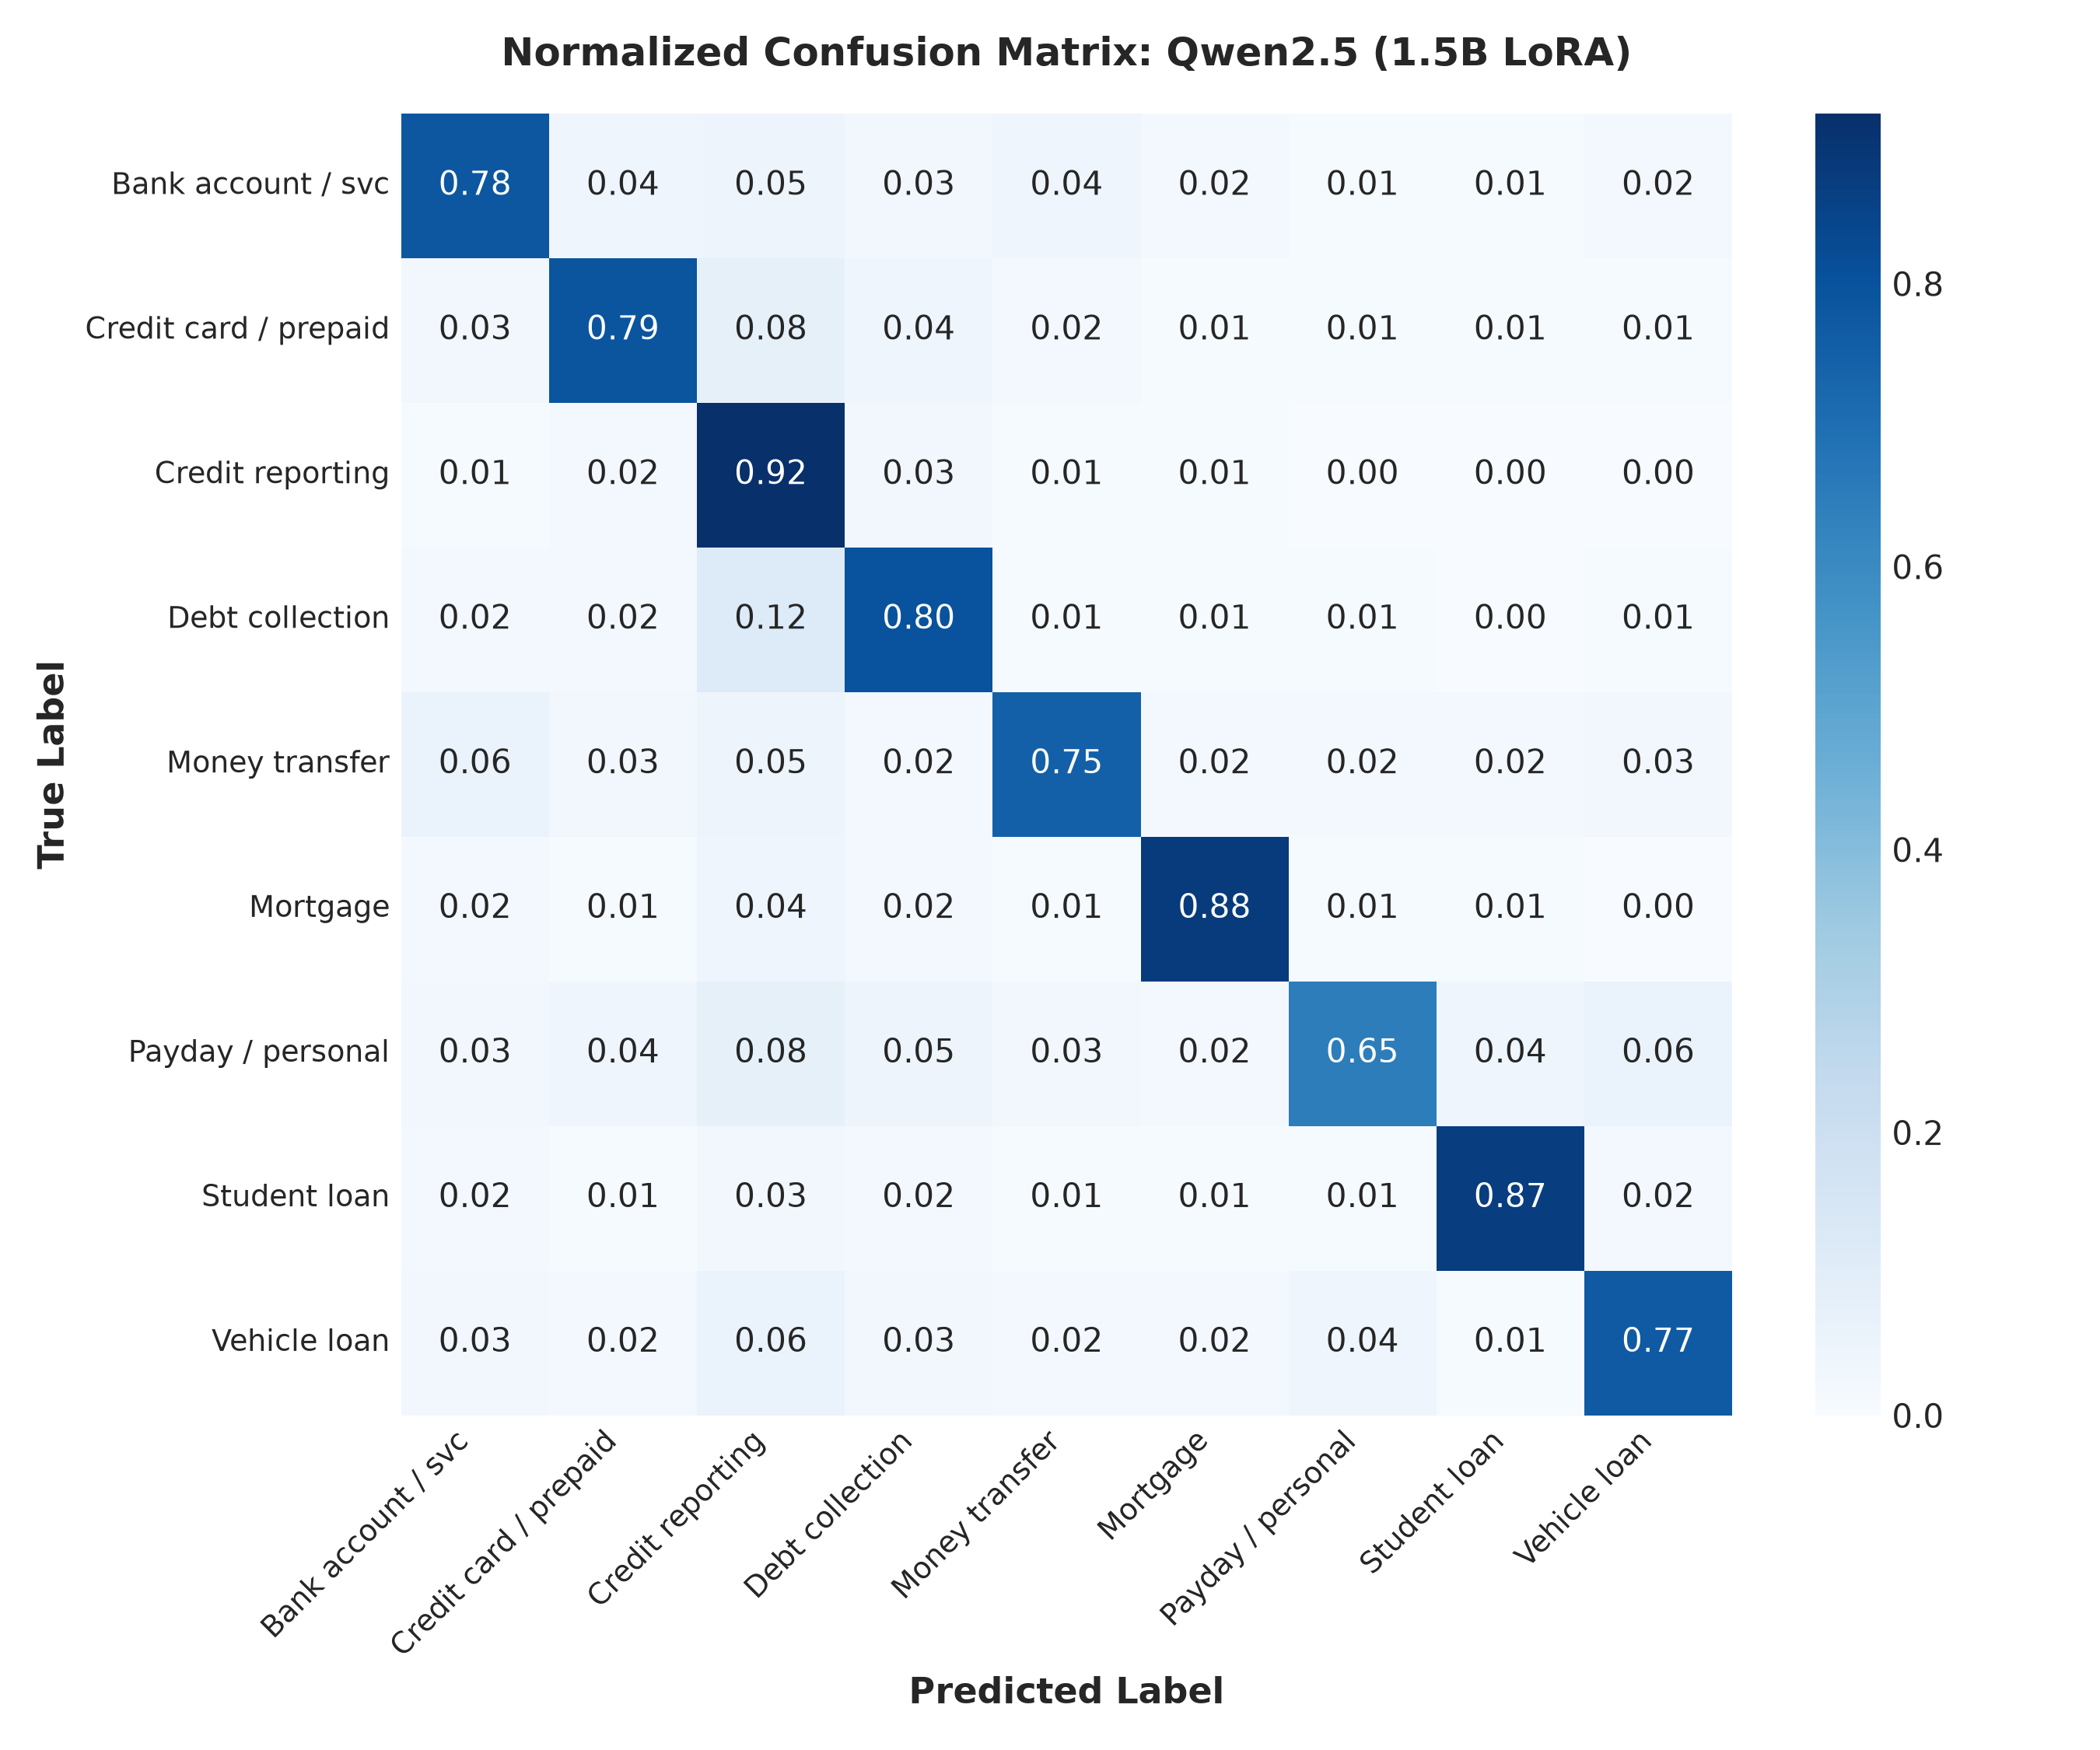
\includegraphics[width=\columnwidth]{figures/qwen_confusion_matrix.png}
\caption{Row-normalised confusion matrix for the Qwen2.5-1.5B LoRA arm on its
5,000-document evaluation subset. Row normalisation makes the diagonal a recall
estimate, which is comparable in shape to the encoder models even though the
scalar metrics are not comparable in level.}
\label{fig:qwencm}
\end{figure}

\subsection{Promoting this arm to the main table}

\texttt{pipeline/qwen\_lora.py} in this repository reproduces the adaptation
above against the shared splits: the same 200,000-row stratified training
budget, the same validation split for epoch selection, and the full
303,213-document test split, with inference timed in the same units as
Table~\ref{tab:main}. Running it writes
\texttt{\_cache/qwen\_lora\_results.json}, including a \texttt{protocol} block
recording the split sizes actually used. Once that file exists, the arm can be
promoted into the main comparison and this appendix retired.


\end{document}
